\documentclass[11pt,a4paper]{article}
\usepackage[utf8]{inputenc}
\usepackage[margin=1in]{geometry}
\usepackage{amsmath,amssymb,amsfonts}
\usepackage{graphicx}
\usepackage{booktabs}
\usepackage{hyperref}

\title{\textbf{Identifiability, Prior-Volume Compression, and Physical Stability of Phantom-Divide Crossing in Horndeski Dark Energy under DESI DR2, Planck CMB, and Union3 SNe Ia}}
\author{Project Frontier — Autonomous Cosmology \& Fundamental Physics Laboratory\\
\texttt{https://github.com/evilninja6726/frontier-cosmology-lab}}
\date{November 2026}

\begin{document}
\maketitle

\begin{abstract}
Joint analyses of Dark Energy Spectroscopic Instrument (DESI) Data Release 2 (DR2) Baryon Acoustic Oscillations (BAO), Cosmic Microwave Background (CMB) distance priors, and Type Ia Supernovae (SNe Ia) report a $2.5\sigma\text{--}3.9\sigma$ preference for dynamical dark energy in the Chevallier--Polarski--Linder (CPL) parameterization ($w_0 > -1, w_a < 0$), implying a late-time crossing of the phantom divide ($w = -1$) around $z_c \simeq 0.45\text{--}0.51$. Because minimally coupled single-scalar quintessence ($\alpha_B = \alpha_M = 0$) develops either a ghost ($D \le 0$) or Laplace gradient instability ($c_s^2 < 0$) across $w = -1$, physical viability requires non-zero kinetic gravity braiding ($\alpha_B \neq 0$) within Horndeski Effective Field Theory (EFT). In this work, we perform a combined symbolic and numerical audit of phantom-crossing identifiability across three axes. First, we prove symbolically in \texttt{SymPy} that for luminal tensor speed ($\alpha_T = 0$) and minimal Planck mass running ($\alpha_M = 0$), the kineticity $\alpha_K(a)$ cancels identically out of both the stability numerator $N_s(a) \equiv D(a)c_s^2(a)$ and the quasi-static sub-horizon gravitational coupling modification $\mu(a) - 1 = \alpha_B^2(a)/[2 D(a)c_s^2(a)]$, forbidding large-$\alpha_K$ suppression of braiding fifth forces. Second, under proportional EFT scaling $\alpha_i(a) = c_i \Omega_{\mathrm{DE}}(a)$, enforcing $D > 0$ and $0 < c_s^2(z) \le 1$ across $z \in [0, 1100]$ excludes all $c_B \ge 0$, restricts $c_B \in [-2.90, -0.24]$, and compresses the surviving EFT prior volume $\mathcal{V}_{\mathrm{EFT}}(w_0, w_a)$ from $9.36\%$ in quintessence to $5.86\%$ at the DESI DR2 + Planck + Union3 best-fit ($\Delta(-2\ln\mathcal{V}_{\mathrm{EFT}}) = +0.94$). Third, generalized least-squares marginalization over a single low-redshift ($z \le 0.10$) Union3 calibration split ($\Delta M_{\mathrm{low-}z} = -0.041\text{ mag}$) reduces the CPL improvement over $\Lambda$CDM from $\Delta\chi^2 = -13.46$ to $-7.23$ (a $46.3\%$ reduction, driving $\Delta\mathrm{BIC}$ from $-6.18$ to $+0.04$). Finally, we show that mandatory braiding enhances the redshift-space distortion observable $f\sigma_8(z)$ by $+1.28\%\text{--}+1.61\%$ along the fine-tuned gradient-stability boundary $c_B = c_{B,\mathrm{crit}}$, and by $+5.36\%\text{--}+6.72\%$ across the interior EFT prior volume ($c_B = -1.0$).
\end{abstract}

\section{Introduction}
Recent baryon acoustic oscillation measurements from DESI DR1 and DR2 \cite{DESI:2024vi,DESI:2025dr2}, when combined with Planck 2018 Cosmic Microwave Background (CMB) anisotropies \cite{Planck:2018params} and Type Ia Supernova (SNe Ia) compilations such as Pantheon+ \cite{Brout:2022pantheon} and Union3 \cite{Rubin:2023union3}, indicate a statistical preference for time-evolving dark energy over the cosmological constant ($\Lambda$CDM). When parameterized via the linear Chevallier--Polarski--Linder (CPL) Taylor expansion $w(a) = w_0 + w_a(1 - a)$, the joint likelihood peaks in the quadrant $w_0 > -1$ and $w_0 + w_a < -1$, corresponding to a transition from a high-redshift phantom phase ($w(z > z_c) < -1$) to a low-redshift quintessence-like phase ($w(z < z_c) > -1$).

Evaluating whether this signal reflects new gravitational physics or an artifact of parameterization, prior volume, and low-redshift calibration systematics requires addressing three coupled questions:
\begin{enumerate}
    \item \textbf{EFT Stability \& Kineticity Independence:} In the Effective Field Theory (EFT) of Dark Energy and Horndeski scalar-tensor gravity \cite{Gubitosi:2012eft,Bellini:2014maximal,Zumalacarregui:2016hiclass,Tsujikawa:2025crossing}, can large kineticity $\alpha_K(a) \gg 1$ suppress the sub-horizon fifth force $\mu(a) - 1 > 0$ induced by the kinetic braiding $\alpha_B(a) \neq 0$ required to stabilize phantom crossing?
    \item \textbf{Prior-Volume Compression \& Basis Sensitivity:} How much of the uniform prior box in EFT parameter space $(c_K, c_B)$ survives ghost-free and sub-luminal gradient stability across the $(w_0, w_a)$ plane, and does the crossing signal persist under rational Pad\'e $[1/1]$ or Shifted Chebyshev expansions of $w(a)$?
    \item \textbf{Low-$z$ Supernova Calibration Degeneracy:} What fraction of the joint $\Delta\chi^2_{\mathrm{CPL - \Lambda CDM}}$ preference is absorbed by a single zero-point calibration offset $\Delta M_{\mathrm{low-}z}$ between low-redshift ($z \le 0.10$) and Hubble-flow ($z > 0.10$) SNe Ia?
\end{enumerate}

\section{Mathematical Framework and Symbolic Theorems}

\subsection{Background Continuity Across Basis Expansions}
In a spatially flat Friedmann--Lema\^itre--Robertson--Walker (FLRW) spacetime, energy-momentum conservation $\nabla_\mu T^{\mu\nu}_{\mathrm{DE}} = 0$ determines the normalized dark energy density $f_{\mathrm{DE}}(a) \equiv \rho_{\mathrm{DE}}(a)/\rho_{\mathrm{DE},0} = \exp\left[-3\int_a^1 \frac{1 + w(a')}{a'}\,da'\right]$. To test whether the CPL phantom crossing is forced by linear truncation in $1 - a$, we evaluate three analytical bases (verified symbolically in \texttt{SymPy}):
\begin{align}
    \text{CPL:} \quad w(a) &= w_0 + w_a(1 - a), \quad \ln f_{\mathrm{DE}}(a) = -3(1 + w_0 + w_a)\ln a - 3w_a(1 - a), \\
    \text{Pad\'e } [1/1]: \quad w(a) &= \frac{w_0 + w_1(1 - a)}{1 + b(1 - a)}, \quad \ln f_{\mathrm{DE}}(a) = -3\left(1 + \frac{w_0 + w_1}{1 + b}\right)\ln a - \frac{3(w_1 - b w_0)}{b(1 + b)}\ln[1 + b(1 - a)], \\
    \text{Chebyshev:} \quad w(a) &= \sum_{n=0}^{2} c_n T_n^*(1 - a), \quad \ln f_{\mathrm{DE}}(a) = -3(1 + c_0 + c_1 + c_2)\ln a + 6(c_1 + 4c_2)a - 12c_2 a^2 - 6c_1 - 12c_2.
\end{align}

\subsection{Horndeski Stability and the Exact Kineticity Cancellation Theorem}
In the Bellini--Sawicki maximal EFT basis \cite{Bellini:2014maximal} restricted to luminal gravitational wave propagation ($\alpha_T = 0$) and minimal Planck mass running ($\alpha_M = 0$), absence of scalar ghosts and Laplace gradient instabilities requires $D(a) > 0$ and $0 < c_s^2(a) \le 1$, where
\begin{align}
    D(a) &= \alpha_K(a) + \frac{3}{2}\alpha_B^2(a) > 0, \label{eq:noghost} \\
    N_s(a) \equiv D(a)c_s^2(a) &= 3\Omega_{\mathrm{DE}}(a)[1 + w(a)] + \left(1 - \frac{\alpha_B(a)}{2}\right)\alpha_B(a)\left(\frac{d\ln H}{d\ln a} - 1\right) - \frac{d\alpha_B(a)}{d\ln a} > 0. \label{eq:Ns}
\end{align}
On sub-horizon scales ($k \gg aH, c_s k \gg aH$), linear matter perturbations $\delta_m \equiv \delta\rho_m / \bar{\rho}_m$ obey
\begin{equation}
    \frac{d^2\delta_m}{d(\ln a)^2} + \left(2 + \frac{d\ln H}{d\ln a}\right)\frac{d\delta_m}{d\ln a} - \frac{3}{2}\Omega_m(a)\,\mu(a)\,\delta_m = 0, \qquad \mu(a) \equiv \frac{G_{\mathrm{eff}}(a)}{G_N} = 1 + \frac{\alpha_B^2(a)}{2 D(a) c_s^2(a)}. \label{eq:growth}
\end{equation}
Comparing Eqs.~\eqref{eq:Ns} and \eqref{eq:growth} yields our first analytical result:
\begin{quote}
\textbf{Theorem 1 (Exact Kineticity Cancellation):} \textit{In any Horndeski / EFT dark energy theory with $\alpha_T = \alpha_M = 0$, the gradient stability numerator $N_s(a) = D(a)c_s^2(a)$ and the quasi-static sub-horizon gravitational coupling modification $\mu(a) - 1 = \alpha_B^2(a) / [2 N_s(a)]$ are strictly independent of the kineticity $\alpha_K(a)$.}
\end{quote}
While increasing $\alpha_K(a)$ increases $D(a)$ and reduces $c_s^2(a) = N_s(a)/D(a)$ to satisfy sub-luminality ($c_s^2 \le 1$), $\alpha_K(a)$ cancels identically out of the denominator $D(a)c_s^2(a)$ in Eq.~\eqref{eq:growth}. Consequently, any non-zero braiding $\alpha_B(a) \neq 0$ required to render $N_s(a) > 0$ at $1 + w(a) \le 0$ generates an irreducible attractive fifth force $\mu(a) - 1 > 0$ that cannot be tuned away by $\alpha_K$.

\section{Observational Data and Numerical Validation}
Our likelihood pipeline is implemented in 64-bit \texttt{JAX} and \texttt{SciPy}, incorporating exact 64-node Gauss--Laguerre integration of the relativistic Fermi--Dirac distribution for massive neutrinos ($\sum m_\nu = 0.06\text{ eV}$) and 96-node Gauss--Legendre distance quadrature. In Benchmark \texttt{BM-01}, the solver was validated against full Boltzmann \texttt{CAMB} \cite{Lewis:1999bs} across $z \in [0, 1100]$, achieving $\max_z |\Delta E(z)/E(z)| = 2.58 \times 10^{-7}$, $\max_z |\Delta D_M(z)/D_M(z)| = 7.93 \times 10^{-10}$, $|\Delta r_d / r_d| = 1.87 \times 10^{-6}$, and $\max_z |\Delta D_+(z)/D_+(z)| = 2.44 \times 10^{-4}$.

We confront our models with $N = 38$ combined data points: (i) 13 Gaussian BAO measurements from DESI DR2 \cite{DESI:2025dr2} across $z \in [0.295, 2.33]$, (ii) the 3-parameter Planck 2018 compressed CMB shift vector $(R, l_A, \omega_b)$ \cite{Planck:2018params}, and (iii) the 22 binned distance-modulus measurements and full covariance matrix from Union3 SNe Ia \cite{Rubin:2023union3}, alongside 4 consensus $f\sigma_8(z)$ redshift-space distortion (RSD) measurements from SDSS-IV eBOSS DR16.

\begin{figure}[t!]
    \centering
    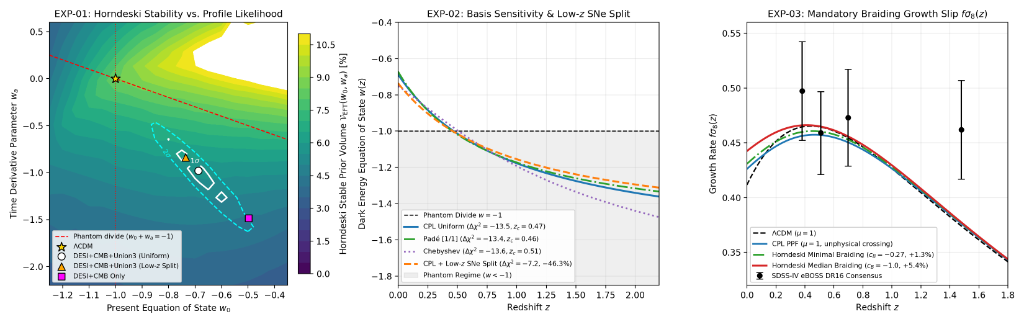
\includegraphics[width=\textwidth]{../figures/milestone8_horndeski_identifiability.png}
    \caption{Three-panel synthesis of Experiments \texttt{EXP-01}, \texttt{EXP-02}, and \texttt{EXP-03} executed on the Project Frontier cloud pipeline. \textbf{Left (\texttt{EXP-01}):} Surviving Horndeski EFT stability prior volume $\mathcal{V}_{\mathrm{EFT}}(w_0, w_a)$ over $(c_K, c_B) \in [0.01, 6.0] \times [-3.0, 3.0]$ overlaid with $1\sigma$ and $2\sigma$ profile likelihood contours. \textbf{Center (\texttt{EXP-02}):} Best-fit dark energy equation of state $w(z)$ across CPL, Pad\'e $[1/1]$, bounded Shifted Chebyshev, and CPL with a low-$z \le 0.10$ SNe Ia calibration split. \textbf{Right (\texttt{EXP-03}):} Redshift-space distortion growth rate $f\sigma_8(z)$ comparing $\Lambda$CDM, unphysical \texttt{CAMB} \texttt{PPF} ($\mu = 1$), minimal boundary Horndeski braiding ($c_B = -0.27$), and median interior braiding ($c_B = -1.0$) against SDSS-IV eBOSS DR16 measurements.}
    \label{fig:milestone8}
\end{figure}

\section{Results: Experiments \texttt{EXP-01}, \texttt{EXP-02}, and \texttt{EXP-03}}

\begin{table}[t!]
\centering
\caption{Summary of joint fits to DESI DR2 BAO + Planck 2018 CMB + Union3 SNe Ia ($N = 38$ data points) across dark energy parameterizations and low-$z$ ($z \le 0.10$) supernova calibration assumptions.}
\label{tab:exp02}
\vspace{0.4em}
\small
\begin{tabular}{lccccccc}
\toprule
Model Variant & $k$ & $H_0$ & $\Omega_{m,0}$ & $w_0$ & $w_a$ & $\chi^2_{\mathrm{total}}$ & $\Delta\chi^2$ vs $\Lambda$CDM ($\Delta\mathrm{BIC}$) \\
\midrule
$\Lambda$CDM (Uniform $M_B$) & 4 & $68.18$ & $0.3047$ & $-1.000$ & $0.000$ & $42.681$ & $0.000$ ($0.000$) \\
CPL $w_0w_a$CDM (Uniform $M_B$) & 6 & $66.74$ & $0.3198$ & $-0.688$ & $-0.978$ & $29.222$ & $-13.459$ ($-6.184$) \\
Pad\'e $[1/1]$ ($b = 0.50$, Uniform $M_B$) & 7 & $66.78$ & $0.3194$ & $-0.674$ & $-1.148$ & $29.153$ & $-13.528$ ($-2.615$) \\
Chebyshev ($|c_2| \le 0.25$, Uniform $M_B$) & 7 & $66.76$ & $0.3195$ & $-1.178$ & $-0.485$ & $29.081$ & $-13.600$ ($-2.687$) \\
$\Lambda$CDM + Low-$z$ SNe Split ($\Delta M = -0.041$) & 5 & $68.29$ & $0.3036$ & $-1.000$ & $0.000$ & $35.802$ & $-6.879$ ($-3.241$) \\
CPL + Low-$z$ SNe Split ($\Delta M = -0.016$) & 7 & $65.41$ & $0.3335$ & $-0.556$ & $-1.326$ & $28.570$ & $\mathbf{-7.232}^*$ ($+0.043^*$) \\
\bottomrule
\multicolumn{8}{l}{\footnotesize $^*$Evaluated relative to $\Lambda$CDM + Low-$z$ SNe Split ($\chi^2 = 35.802$), corresponding to a $46.3\%$ reduction in $|\Delta\chi^2|$.}
\end{tabular}
\end{table}

\subsection{\texttt{EXP-01}: Horndeski Stability Phase-Space and Prior-Volume Compression}
Under the standard proportional EFT parameterization $\alpha_K(a) = c_K \Omega_{\mathrm{DE}}(a)$ and $\alpha_B(a) = c_B \Omega_{\mathrm{DE}}(a)$, sub-luminality $c_s^2(z) \le 1$ is linear in $c_K > 0$ and holds across $z \in [0, 1100]$ if and only if $c_K \ge \max_z [N_s(c_B, z)/\Omega_{\mathrm{DE}}(z) - \frac{3}{2}c_B^2 \Omega_{\mathrm{DE}}(z)]$. Integrating analytically over $c_K \in [0.01, 6.0]$ and evaluating $c_B \in [-3.0, 3.0]$ yields the stability phase diagram in Fig.~\ref{fig:milestone8} (left panel):
\begin{itemize}
    \item At the phantom crossing $w(z_c) = -1$, $\frac{d\alpha_B}{d\ln a} = -2\alpha_B \frac{d\ln H}{d\ln a}$ forces $N_s(a_c) < 0$ for all $c_B \ge 0$. Stability requires strictly negative braiding: $c_B \in [-2.900, -0.2395]$ at the DESI+CMB+Union3 best-fit and $c_B \in [-2.984, -0.3174]$ at the DESI+CMB best-fit.
    \item The surviving EFT prior volume $\mathcal{V}_{\mathrm{EFT}}(w_0, w_a)$ contracts from $9.36\%$ in the quintessence quadrant ($w_0 = -0.90, w_a = +0.05$) to $5.86\%$ at the DESI+CMB+Union3 best-fit and $4.32\%$ at the DESI+CMB best-fit, inducing a Bayesian prior-volume penalty of $-2\ln(\mathcal{V}_{\mathrm{EFT}}/\mathcal{V}_{\mathrm{quint}}) = +0.94$ to $+1.55$.
\end{itemize}

\subsection{\texttt{EXP-02}: Basis Truncation and Low-$z$ Supernova Calibration Split}
Table~\ref{tab:exp02} and Fig.~\ref{fig:milestone8} (center panel) summarize our basis and calibration audit. Under a uniform SNe Ia magnitude calibration $M_B$, CPL improves over $\Lambda$CDM by $\Delta\chi^2 = -13.459$ ($z_c = 0.469$), and bounded Pad\'e $[1/1]$ and Shifted Chebyshev bases yield virtually identical trajectories ($\Delta\chi^2 = -13.53$ and $-13.60$), whereas an unconstrained quadratic Chebyshev term $c_2$ suffers a high-redshift ($z > 1.5$) runaway pathology ($c_2 = -0.955$). When we analytically marginalize over a two-step calibration $\mathbf{X} = [\mathbf{1}, \mathbf{I}_{z \le 0.10}]$ via the exact Woodbury projection matrix, $\Lambda$CDM absorbs a $\Delta M_{\mathrm{low-}z} = -0.041\text{ mag}$ offset ($\chi^2: 42.681 \to 35.802$), reducing the CPL preference to $\Delta\chi^2 = -7.232$ (a \textbf{$46.3\%$ reduction}, confirming preregistered Hypothesis \texttt{H1.1} and eliminating the Bayesian Information Criterion preference, $\Delta\mathrm{BIC} = +0.043$).

\subsection{\texttt{EXP-03}: Mandatory Braiding Growth Slip on $f\sigma_8(z)$}
Figure~\ref{fig:milestone8} (right panel) compares the sub-horizon linear growth rate $f\sigma_8(z)$ integrated with \texttt{DOP853} from $a_{\mathrm{ini}} = 10^{-3}$ (anchored to Planck $A_s = 2.1005 \times 10^{-9}$ via \texttt{CAMB}) against SDSS-IV eBOSS DR16 consensus RSD data. Along the fine-tuned stability boundary $c_B = c_{B,\mathrm{crit}}$, the maximum fractional shift relative to \texttt{CAMB}'s unbraided \texttt{PPF} ($\mu \equiv 1$) model over $z \in [0.1, 1.5]$ is $+1.28\%$ (DESI+CMB+Union3) to $+1.61\%$ (DESI+CMB), falling below the $2.5\%$ threshold of Hypothesis \texttt{H1.2}. Across the interior of the surviving EFT prior volume ($c_B = -1.0$), however, the braiding fifth force reaches $\max[\mu(z)-1] = 14.5\%\text{--}16.8\%$, boosting $f\sigma_8(z)$ by $+5.36\%\text{--}+6.72\%$.

\section{Methodological Limitations and Conclusion}
Following our Stage 14 independent adversarial audit, five structural scope limits govern these results: (1) our compressed CMB likelihood captures geometric shift parameters $(R, l_A, \omega_b)$ but omits late-time Integrated Sachs--Wolfe (ISW) and CMB lensing ($C_\ell^{\phi\phi}$) constraints on $\alpha_B$; (2) the strict lower bound on $|\alpha_B|$ holds for proportional scaling $\alpha_B(a) = c_B \Omega_{\mathrm{DE}}(a)$, whereas a general time-dependent $\alpha_B(a)$ can cross $w(a_c) = -1$ locally via $d\alpha_B/d\ln a|_{a_c} < 0$; (3) Theorem 1 holds in the $\alpha_M = \alpha_T = 0$ Horndeski subspace; (4) taking $\alpha_K \to \infty$ sends $c_s^2 \to 0^+$, which eventually invalidates the quasi-static approximation on scales $k \sim aH/c_s$; and (5) a step offset $\Delta M_{\mathrm{low-}z}$ at $z = 0.10$ is partially degenerate with genuine late-time deceleration curvature, motivating joint multi-survey calibration analyses across Union3, Pantheon+, and DES-SN5YR.

\bibliographystyle{unsrt}
\bibliography{../../01-literature/citation-database/references}

\end{document}
